\section{El paquete de Python y los bloques que lo conforman}
Python es un lenguaje de código abierto, con una comunidad activa de colaboradores y usuarios que comparten su software para que otros desarrolladores lo utilicen. Son colaboradores, aquellos que comparten sus códigos o scripts, en forma de paquetes en el Python Packaging Index (PyPI). Los paquetes son similares a directorios de un sistema de archivos, ya que estos permiten separar el código de forma jerárquica \cite{Paquetes}. 
\subsection{Módulos}
Se conoce como modulo a todo fichero o script de Python cuya extensión es .py. Separar el código en módulos permite facilitar el mantenimiento del programa a medida que crezca. Algunos aspectos a tomar en cuenta sobre los módulos serían:
\begin{itemize}
    \item Pueden contener tanto declaraciones ejecutables como definiciones de funciones. Estas declaraciones están pensadas para inicializar el módulo. Se ejecutan únicamente la primera vez que el módulo se encuentra en una declaración import\cite{ModuloPython}.
    \item Cada módulo tiene su propio espacio de nombres, el cual es usado como espacio de nombres global para todas las funciones definidas en su interior.
\end{itemize}
\subsection{Tipos de scripts de configuración del paquete}
\subsubsection{Distutils}
Es un paquete de Python que da soporte, para la creación, distribución e instalación de módulos, los módulos pueden ser hechos únicamente en Python o escritos en C. Distutils como paquete presenta las siguientes funcionalidades:
\begin{itemize}
    \item Soporte para declarar dependencias del proyecto, siendo las dependencias aquellos paquetes o módulos externos necesarios para el funcionamiento del proyecto.
    \item Mecanismos adicionales para configurar cuáles archivos incluir en lanzamientos de código fuente, esto se logra mediante el uso de sistemas de control de versiones.
    \item La capacidad de generar, automáticamente, ejecutables de línea de comandos de Windows en el momento de la instalación, en lugar de tener que compilarlos previamente.
    \item Comportamiento consistente en todas las versiones de Python soportadas por el paquete.
\end{itemize}
Un ejemplo de como estructurar el archivo setup.py que maneja Distutils sería:
\begin{figure}[H]
    \centering
    \begin{minted}{Python}
		from distutils.core import setup
		setup(name='Distutils',
                version='1.0',
                description='Python Distribution Utilities',
                author='Greg Ward',
                author_email='gward@python.net',
                url='https://www.python.org/sigs/distutils-sig/',
                packages=['distutils', 'distutils.command'],)
	\end{minted}
    \caption{Ejemplo de archivo setup.py utilizando el paquete Distutils}
    \label{ejDistutils}
\end{figure}
En la Figura \ref{ejDistutils} es importante resaltar la opción ``packages'' debido a que esta le dice a Distutils que procese (compile, distribuya, instale, etc.) todos los módulos de Python que se encuentran en cada paquete mencionado en la lista de "packages".
\subsubsection{Setuptools}
Es un paquete que contiene una serie de mejoras a las capacidades de Distutils, cuya cualidad principal es permitir que los desarrolladores puedan distribuir paquetes de forma más sencilla, con especial énfasis en paquetes que posean dependencias externas. Esto no implica que distutils sea obsoleto, puesto que setuptools aún se encuentra en desarrollo. A diferencia de su contra parte, las configuraciones requieren de al menos 2 archivos y un paquete, el archivo pyproject.toml; es aquel donde se debe declarar que se empleara Setuptools, este archivo debe poseer la siguiente estructura:
\begin{figure}[H]
    \centering
    \begin{minted}{Python}
		[build-system]
        requires = ["setuptools", "wheel"]
        build-backend = "setuptools.build_meta"
	\end{minted}
    \caption{Ejemplo de archivo pyproject.toml}
    \label{pyproject.toml}
\end{figure}
El archivo setup.cfg es el reemplazo al archivo setup.py y puede conformarse de la siguiente manera:
\begin{figure}[H]
    \centering
    \begin{minted}{Python}
		[metadata]
        name = "mypackage"
        version = 0.0.1

        [options]
        packages = "mypackage"
        install_requires =
        requests
        importlib; python_version == "2.6"
        
        [options.entry_points]
        console_scripts =
        main = mypkg:some_func
	\end{minted}
    \caption{Ejemplo de archivo setup.cfg}
    \label{setup.cfg}
\end{figure}
Como se puede ver en la Figura \ref{setup.cfg} el archivo es bastante similar en estructura al fichero setup.py; no obstante, tiene varias ventajas, ya que los elementos que pertenecen a la opción \mintinline{Python}{install_requires}, son directamente las dependencias del paquete, e incluso al momento de instalar un paquete externo, setuptools actualiza las dependencias necesarias. Para proyectos muy grandes es posible automatizar la búsqueda de paquetes, con el fin de que no sea necesario declarar cada paquete en el fichero setup.cfg. 
Las herramientas de configuración admiten la creación automática de scripts tras la instalación mediante "\mintinline{Python}{options.entry_points}". Un paquete que emplee setuptools debe poseer la siguiente estructura de directorios:
\begin{figure}[H]
    \centering
    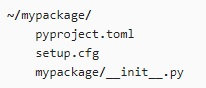
\includegraphics{Recursos/estructuraSetupTools.jpg}
    \caption{Estructura de paquete mediante setuptools}
    \label{estructuraSetupTools}
\end{figure}
El último elemento que requiere Setuptools es el paquete pep517, el cual se puede instalar mediante el instalador de paquetes de python "pip", posteriormente se debe invocar con el comando \mintinline{Python}{python -m pep517.build}.
\subsection{El paquete wheel}
Es un proyecto compatible con distutils y setuptools, que produce un formato de empaquetado binario multiplataforma (llamado ``wheels'' o ``wheel files'' y definido en PEP 427) es decir; la función de wheels es permitir la distribución de paquetes sin importar el sistema operativo empleado \cite{wheel}.
\subsection{Pruebas de regresión mediante módulo unittest}
El objetivo de las pruebas de regresión implementadas mediante el módulo unittest, es probar situaciones donde el código deje de funcionar, para encontrar errores en el mismo y solventar problemas en el software, de acuerdo con la documentación oficial existen una serie de pautas a seguir para ejecutar dichas pruebas, las más importantes en el caso del software a desarrollar son:
\begin{itemize}
    \item El conjunto de pruebas se debe hacer a todas las clases, funciones y constantes.
    \item Importar la menor cantidad de módulos posible. Esto minimiza las dependencias externas de las pruebas y también minimiza el posible comportamiento anómalo de los efectos secundarios de importar un módulo.
    \item Maximizar la reutilización del código. En ocasiones, las pruebas variarán en algo tan pequeño como qué tipo de entrada se utiliza.
    \item Asegurar la limpieza después de las pruebas (así como cerrar y eliminar todos los archivos temporales).
    \item Asegurar que todos los valores posibles son probados, incluidos los no válidos. Esto permite que no solo todos los valores válidos sean aceptables, sino que los valores incorrectos se manejen correctamente.
    \item Añadir una prueba explícita para cualquier error descubierto para el código probado. Esto asegurará que el error no vuelva a aparecer si el código se cambia en el futuro.
\end{itemize}
\subsection{Pruebas integradas en cadenas de caracteres de documentación mediante módulo doctest}
Este módulo busca fragmentos de código comentado en el fichero y luego ejecuta esas secciones para verificar que funcionan exactamente como se muestran. Hay varias formas comunes de usar doctest:
\begin{itemize}
    \item Para comprobar que las cadenas de documentación de un módulo estén actualizadas, verificando que todos los ejemplos interactivos sigan funcionando como se documenta.
    \item Para realizar pruebas de regresión verificando que los ejemplos interactivos de un archivo de prueba o un objeto de prueba funcionen como se espera. Esto implica que doctest no sustituye al módulo unittest, al contrario cuando se emplean en conjunto es posible automatizar las pruebas realizadas por doctest.
    \item Para escribir documentación didáctica para un paquete, ilustrada abundantemente con ejemplos de entrada y salida.
\end{itemize}
\section{Proceso de visión estereoscópica}
 En general la visión estéreo consiste en recuperar las características tridimensionales de una escena a partir de múltiples imágenes tomadas desde varios puntos de vista. De acuerdo con lo propuesto por Barnard y Fischler en 1982, las investigaciones sobre soluciones computacionales para la generalización del problema estéreo siguen un simple paradigma \cite{Barnard1982}, el cual involucra los siguientes pasos:
\subsection{Adquisición de imágenes}
Esta etapa engloba las condiciones externas del entorno, como la iluminación y el campo o dominio de aplicación, ya que; no es igual captar imágenes en entornos cerrados donde la iluminación puede ser constante, en comparación con entornos abiertos donde esta cambiará en el transcurso del día. Las condiciones climáticas pueden influir en la calidad de la imagen, la existencia de oclusión puede afectar al momento de interpretar las imágenes y posteriormente realizar satisfactoriamente el paso de correspondencia. El posicionamiento relativo entre cámaras es un factor a tomar en cuenta, dado que este modifica los modelos utilizados en el sistema y su posterior procesamiento.
\\
Hasta el momento se han mencionado únicamente los factores externos, sin embargo; al adquirir imágenes estos no son los únicos a tener en cuenta; tal es el caso, del tiempo en que se toman las muestras de cada imagen, el cual dependerá de las especificaciones técnicas del hardware empleado, puesto que este posee limitaciones en cuanto a velocidad de transmisión y procesamiento, entre otros aspectos ligados a los instrumentos, se encuentra la resolución; que esta asociada al campo de aplicación, otro factor sería; el campo de visión o field of view (FOV), que no es más que el ángulo abarcable por el sensor de una cámara. Además hay ocasiones en las que el ruido (provocado por el sensor de la cámara) presente en las imágenes es reducido mediante un preprocesamiento para así mejorar el resultado final del sistema.
\subsection{Modelado de la cámara (geometría del sistema)}
Es una representación de los atributos geométricos y físicos más importantes de las cámaras. Para poder representar los modelos de las cámaras se emplea el sistema de coordenadas homogéneas y la matriz homogénea, esta es una herramienta introducida por Forest en 1969 para resolver diferentes problemas de gráficos por computador a través de operaciones con matrices. Este tipo de transformaciones son empleadas para determinar en una sola matriz la posición y orientación de un objeto respecto a un sistema de referencia \cite{RSSFernando_homogeneusC}.

Cuando se emplean coordenadas homogéneas en imágenes, cada píxel tiene la siguiente representación:
\begin{equation}
(x, y) \Rightarrow
\begin{bmatrix}
x & y & 1
\end{bmatrix}^{T}
\end{equation}
Mientras que en el caso de una escena tridimensional la representación es:
\begin{equation}
(x, y, z) \Rightarrow
\begin{bmatrix}
x & y & z & 1
\end{bmatrix}^{T}
\end{equation}
Las traslaciones y rotaciones para las coordenadas homogéneas son operaciones lineales realizadas entre matrices, donde la nueva posición de un objeto, será el producto entre la posición previa y la matriz de transformación. La matriz de transformación homogénea definida por Forest es de dimensiones 4x4 y está compuesta a su vez por cuatro submatrices (Ecuación \ref{homogeneusMatrix}).
\begin{equation}
    T = \begin{bmatrix}
        \begin{array}{c|c}
                rotaci\acute{o}n & traslaci\acute{o}n\\
                \hline
                perspectiva & escalado
        \end{array}
        \end{bmatrix}
        =
        \begin{bmatrix}
        \begin{array}{c|c}
                3 x 3 & 3 x 1\\
                \hline
                1 x 3 & 1 x 1
        \end{array}
        \end{bmatrix}
\label{homogeneusMatrix}
\end{equation}
No obstante la matriz de transformación en el plano imagen es de dimensiones 3 x 3 y tiene la siguiente representación:
\begin{equation}
    T = \begin{bmatrix}
        \begin{array}{c|c}
                rotaci\acute{o}n & traslaci\acute{o}n\\
                \hline
                perspectiva & escalado
        \end{array}
        \end{bmatrix}
        =
        \begin{bmatrix}
        \begin{array}{c|c}
                2 x 2 & 2 x 1\\
                \hline
                1 x 2 & 1 x 1
        \end{array}
        \end{bmatrix}
\end{equation}
Cuando se emplean coordenadas homogéneas no solo es más eficaz a nivel computacional, ya que permite efectuar cambios en la posición y orientación mediante productos matriciales e incluso se pueden convertir en coordenadas convencionales mediante una simple operación de división tal que:
\begin{align}
\begin{bmatrix}
x & y & w
\end{bmatrix}^{T} \Rightarrow (x/w, y/w)\label{homogeneus2d}\\
\begin{bmatrix}
x & y & z & w
\end{bmatrix}^{T} \Rightarrow (x/w, y/w, z/w)\label{homogeneus3d}
\end{align}
La ecuación \ref{homogeneus2d} se utiliza para convertir un píxel de una imagen 2D que se encuentra en coordenadas homogéneas a cartesianas, mientras que la ecuación \ref{homogeneus3d} se utiliza en el caso de tres dimensiones.
\\
Para poder estudiar un modelo de múltiples cámaras, es menester comprender como se aplican las coordenadas homogéneas en el caso de una sola cámara. Por este motivo a continuación se presentará el ``modelo de pinhole'', el cual consiste en que cada punto de un objeto situado en el entorno de trabajo (espacio tridimensional) se proyecta en un punto de un plano denominado plano imagen ó plano de proyección. En la Figura \ref{pinholeModel} ``PP'' es el plano de proyección y ``COP'' se refiere al centro de proyección o centro óptico de la cámara. El punto en la escena 3D se denota como $p^{M}$, dicho punto se encuentra en las coordenadas del mundo $p^{M}$ $(x, y, z)$ y su proyección en el plano de imagen se denota como $p^{I}$ $(x', y')$ y corresponde con la intersección entre la línea que une $p^{M}$ y COP con el plano de imagen, además a la distancia entre el plano de proyección y COP se le conoce como distancia focal. 
\begin{figure}[H]
    \centering
    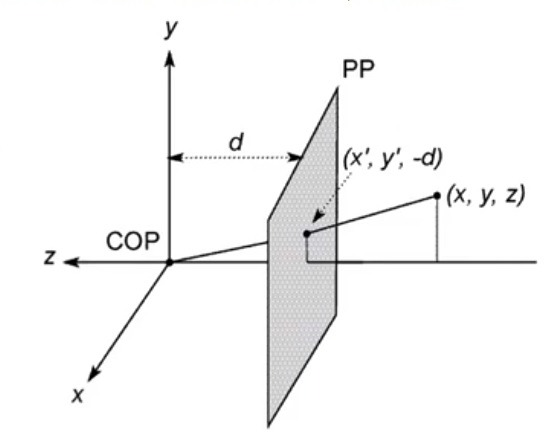
\includegraphics[scale=0.5]{Recursos/pinholeModel.jpg}
    \caption{Modelo de cámara pinhole}
    \label{pinholeModel}
\end{figure}
La razón del porqué en el modelo presentado en la Figura \ref{pinholeModel} el plano de proyección se encuentra por delante del lente (a pesar de que en la realidad la luz ingresa a través del punto focal y luego impacta con el plano de imagen) es debido a que matemáticamente es más conveniente, porque de esta forma las imágenes no son invertidas.

Utilizando el teorema de Tales es posible determinar las proyecciones de los puntos en el plano de forma tal que se cumple la siguiente ecuación:
\begin{equation}
    (X, Y, Z) \longrightarrow (-d\frac{X}{Z}, -d\frac{Y}{Z}, -d)  \label{convert3Dto2Dpinhole}
\end{equation}
La operación realizada por la ecuación \ref{convert3Dto2Dpinhole}, permite proyectar los puntos del espacio 3D en el plano de imagen, dicha operación puede ser realizada mediante coordenadas homogéneas de la siguiente forma:
\begin{align}
            \begin{bmatrix}
            1 & 0 & 0 & 0\\
            0 & 1 & 0 & 0\\
            0 & 0 & 1/f & 0
            \end{bmatrix}
            \begin{bmatrix}
            x\\
            y\\
            z\\
            1
            \end{bmatrix}
            =
            \begin{bmatrix}
            x\\
            y\\
            z/f\\
            \end{bmatrix} \Rightarrow \left(-f\frac{X}{Z}, -f\frac{Y}{Z}\right)\label{convert3Dto2Dperspective}
\end{align}
A la forma en la que se proyecta en la ecuación \ref{convert3Dto2Dperspective} se le conoce como proyección de perspectiva y esta llega al mismo resultado que el de la ecuación \ref{convert3Dto2Dpinhole}, ya que $f$ y $d$ son la distancia focal. Aunque la transformación presente en la ecuación \ref{convert3Dto2Dperspective} es válida, el enfoque más común para determinar el modelo de una cámara utiliza al menos 11 parámetros, en la sección siguiente se detallara al respecto.
\subsubsection{Calibración de la cámara}\label{calibration_section}
Para modelar una cámara y así localizar un objeto del mundo real (espacio tridimensional) a partir de imágenes es necesario recuperar información que se pierde al pasar del espacio 3D al plano de imagen. La información perdida corresponde con los parámetros que intervienen en el proceso de formación de imágenes, los cuales se definen como:
\begin{itemize}
\item \textbf{Parámetros intrínsecos:} son los que describen la geometría y óptica del sensor. Engloban el proceso desde que un rayo alcanza la lente del objetivo hasta que impresiona un elemento sensible.
\item \textbf{Parámetros extrínsecos:} son aquellos que definen la orientación y posición de la cámara respecto a un sistema de coordenadas conocido al que se llama sistema del mundo. Se representa con una matriz 3 x 4, donde las primeras 3 columnas corresponden con la submatriz de rotación y la última es la submatriz de translación. Posee 3 grados de libertad para la orientación y 3 que definen el desplazamiento.
\end{itemize} 
Los parámetros intrínsecos y extrínsecos de una cámara, permiten convertir un punto que se encuentre en el sistema de referencia del mundo $p^{M}$ al plano de imagen $p^{I}$ y viceversa. A continuación se presenta la forma en la que se realiza dicha transformación:
\begin{align}
    p^{I} = M p^{w} \\
    p^{I} = M \begin{bmatrix}
            x & y & z & 1
            \end{bmatrix}^{T} \\
    p^{I} = K \begin{bmatrix}R & T\end{bmatrix} \begin{bmatrix}
            x & y & z & 1
            \end{bmatrix}^{T}  \label{point_projection}
\end{align}
En la ecuación \ref{point_projection} la matriz K de dimensiones 3x3 representa los parámetros intrínsecos, por lo que la matriz que involucra la rotación y traslación del sistema corresponde con los parámetros extrínsecos. Existen diversos métodos de calibración que permiten hallar algunos o todos los parámetros necesarios para realizar la transformación de coordenadas 3D a 2D, pero de todas las estrategias, la más empleada, es la propuesta por Zhengyou Zhang \cite{Zhang2000}, la cual sigue los siguientes pasos para obtener ambas matrices:
\begin{enumerate}
\item Se imprime un patrón (es común que el patrón sea en forma de tablero de ajedrez) y se adhiere sobre una superficie plana.
\item Se capturan $n$ imágenes del plano de ajedrez, donde $n$ suele variar entre 15 y 20.
\item Se detectan las esquinas internas en cada imagen de cada tablero. En el caso de ser un patrón circular se detectaran los centros de cada punto de calibración.
\item Se estiman los parámetros intrínsecos y extrínsecos usando la solución cerrada propuesta por Zhengyou Zhang \cite{Zhang2000}
\item Se refina el cálculo de los parámetros incluyendo la distorsión generada por la lente de la cámara. Es importante recalcar, que este es un proceso iterativo, emplea el criterio de máxima verosimilitud para así alcanzar el valor más óptimo, por lo que puede darse el caso de que dependiendo del número de imágenes o las posiciones en las que fue capturado el tablero, la solución no converja a un valor que minimice el error.
\end{enumerate}
\subsubsection{Modelo de dos cámaras}
El modelo de dos cámaras o modelo estéreo, es una extrapolación del modelo de pinhole. En general se pueden tener 3 casos en función de cómo se encuentren orientados los ejes de ambas cámaras: disposición convergente, disposición alineada y la disposición divergente, la tercera no permite llevar a cabo un análisis estéreo. En la figura \ref{epipolar_geometry}, se puede observar el modelo geométrico de dos cámaras cuando sus ejes ópticos son convergentes, a continuación se listan cada uno de los elementos relevantes:
\begin{itemize}
\item \textbf{Linea base:} es la distancia que separa los dos centros ópticos de ambas cámaras. En la Figura \ref{epipolar_geometry} se asocia a la línea naranja y se identifica con la letra $B$.
\item \textbf{distancia focal:} la distancia entre el plano de imagen y los centros ópticos. Se denota $f$.
\item\textbf{El punto P:} corresponde con la distancia Z en las coordenadas de los sistemas de cámaras, siempre es medida hasta el centro de proyección ($COP$ ó $O$) de cada cámara. 
\item \textbf{Plano epipolar de un punto P en el espacio:} en la Figura \ref{epipolar_geometry} es el plano conformado por los puntos $P$, $O_{1}$ y $O_{2}$.
\item\textbf{Línea epipolar:} hay una por cada punto ($p$ y $p'$), en el caso de la Figura \ref{epipolar_geometry}, corresponde con la intersección del plano epipolar y cada plano de imagen, a su vez, esta contiene la proyección del punto y el epipolo.
\item\textbf{Epipolo:} Hay uno por cada cámara ($e$ y $e'$). Es la proyección sobre una cámara del centro óptico de la otra cámara. En el epipolo confluyen todas las líneas epipolares. En el caso de una disposición alineada no se representan los epipolos, ya que estos se encuentran en el infinito.
\end{itemize}
\begin{figure}[H]
    \centering
    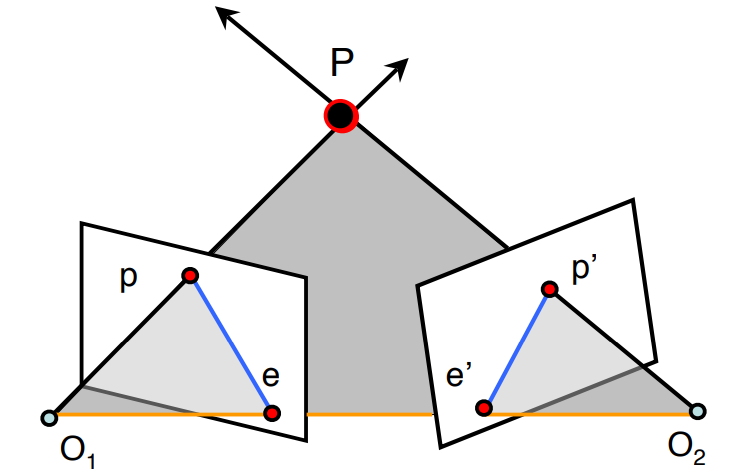
\includegraphics[scale=0.3]{Recursos/epipolar_geometry.png}
    \caption{Disposición convergente de la geometría epipolar}
    \label{epipolar_geometry}
\end{figure}
El potencial de la geometría epipolar está en que para todo píxel $p$ solo puede corresponder una proyección $p'$, la cual siempre estará situada a lo largo de una línea epipolar, definida por el epipolo $e'$ y la proyección $p'$. Esta restricción permite reducir considerablemente el espacio de búsqueda de proyecciones correspondientes en la otra imagen a una sola dimensión. Para poder aprovechar las ventajas de la geometría epipolar a nivel computacional, se utiliza el álgebra de la siguiente forma: asumiendo que un punto P en el sistema del mundo se proyecta en ambos planos de imagen como $p$ y $p'$ la representación de una proyección respecto a la otra es tal que
\begin{equation}
    p' = Rp + T
\end{equation} 
donde $R$ es la matriz de rotación que indica los ángulos de rotación de una cámara respecto a otra y T es la matriz de traslación entre ambas ó la línea base del sistema. Si se aplica el producto cruz de T en ambos lados de la expresión se tiene que:
\begin{equation}
    T \times p' = T \times Rp + T \times T
\end{equation}
De la expresión previa $T \times p'$ es perpendicular al plano epipolar y $T \times T$ es 0, de modo que:
\begin{align}
    T \times p' = T \times Rp
\end{align}
Aplicando el producto escalar de $p'$
\begin{align}
    p'\cdot(T \times p') = p' \cdot(T \times Rp)\\
    0 = p' \cdot(T \times Rp)
\end{align}
Y substituyendo $E$ = $T \times R$, se tiene que:
\begin{equation}
    p'^{T} \cdot(Ep) = 0 \label{esential_eq}
\end{equation}
En la expresión \ref{esential_eq} $E$ es conocida como la matriz esencial y esta depende únicamente de la disposición del sistema de adquisición de datos, dicha ecuación indica que si se tiene un punto en una imagen de un conjunto de cámaras calibradas, existirá una línea en la otra imagen sobre la cual reposara la proyección de dicho punto. En una disposición de cámaras alineadas la única diferencia en la matriz esencial es que la matriz $R$ es igual a la identidad, por lo que el producto vectorial $T \times R$ se simplifica.
\\
\\
Por medio de la matriz esencial es posible reducir el problema de correspondencia en el modelo estéreo; sin embargo, esta metodología presenta el inconveniente de que ambas cámaras sean calibradas, por lo tanto para conocer la geometría epipolar sin calibrar el sistema, se selecciona un conjunto de puntos y sus correspondencias en cada cámara, cuya representación en el plano de imagen coincide con la expresión \ref{point_projection} y a partir de dicha expresión se tiene que un punto en el plano de imagen respecto al marco referencial de la cámara está dado por:
\begin{equation}
    p^{I} = Kp^{c}
\end{equation}
La matriz K es invertible por lo que es posible expresar el caso contrario de la siguiente forma
\begin{equation}
    p^{c} = K^{-1}p^{I} \label{point_in_camera_frame}
\end{equation}
La expresión \ref{point_in_camera_frame} aplicada a ambas cámaras sería:
\begin{align}
    p_{c,l} = K^{-1}_{l}p^{I}_{l}\\
    p_{c,r} = K^{-1}_{r}p^{I}_{r}
\end{align}
Y para poder relacionar las dos ecuaciones previas, se hace uso de la expresión \ref{esential_eq} que relaciona ambas proyecciones de un punto, de modo que:
\begin{align}
    p_{c,r}^{T} E p_{c,l} = 0\\
    (K^{-1}_{r}p^{I}_{r})^{T}E(K^{-1}_{l}p^{I}_{l}) = 0\\
    (p^{I}_{r})^{T}((K^{-1}_{r})^{T}EK^{-1}_{l})p^{I}_{l} = 0\\
    F = (K^{-1}_{r})^{T}EK^{-1}_{l} \label{fundamental_matrix} \\
    (p^{I}_{r})^{T}Fp^{I}_{l} = 0 \label{fundamental_eq}
\end{align}
En la expresión \ref{fundamental_eq} $F$ corresponde con la matriz fundamental la cual se define en la ecuación \ref{fundamental_matrix}, esta depende únicamente de la matriz esencial y los parámetros internos de ambas cámaras, además posee las siguientes propiedades:
\begin{itemize}
    \item Si $p^{T}Fp'$ = 0, se tiene que la expresión $l$ = $Fp'$ es la línea epipolar en la imagen que contiene a $p$, la cual esta asociada a la proyección $p'$. Similar al caso previo $l'$ = $F^{T}p$ es la línea epipolar en la imagen que contiene a $p'$, la cual se asocia a la proyección $p$.
    \item Los epipolos en ambos planos de imagen pueden ser hallados resolviendo las expresiones $Fp'$ = 0 y $F^{T}p$ = 0.
    \item La matriz fundamental $F$ posee dimensiones 3 x 3 y es singular.
\end{itemize}
En síntesis la matriz fundamental relaciona las coordenadas de los píxeles en dos vistas o planos de imagen y es más general que la matriz esencial debido a que remueve la necesidad de requerir una calibración previa, ya que es posible estimar la matriz fundamental, a partir de las correspondencias de las coordenadas de los píxeles y así reconstruir la geometría epipolar sin conocer los parámetros intrínsecos y extrínsecos.
\subsubsection{Rectificación del modelo}
De acuerdo con Richard I. Hartley el método de rectificación de imágenes, es un proceso que remuestrea un par de imágenes estéreo tomadas desde diferentes puntos de vista para así producir un par de proyecciones epipolares coincidentes. Estas son
proyecciones en las que las líneas epipolares corren paralelas al eje x, y en consecuencia las disparidades estarán únicamente en la dirección de dicho eje. Su método se basa en el análisis de la matriz fundamental de Longuet-Higgins la cual describe la geometría epipolar. Esta aproximación utiliza métodos basados en proyección geométrica para así determinar un par de transformaciones en 2D que permitan convertir un sistema de disposición convergente uno de disposición alineada \cite{Hartley1999}.
\subsection{Correspondencia de las imágenes}
La finalidad de la correspondencia, es calcular el grado de disparidad existente entre las localizaciones de las proyecciones en cada imagen, para así convertir dicha disparidad en la profundidad y recuperar la información perdida en el proceso de captación de imágenes, la disparidad puede ser representada de la siguiente forma:
\begin{equation}
d = x_{l} - x_{r} = \frac{f\cdot B}{z_{p}}
\end{equation}
Existen dos formas de correspondencia la dispersa y la densa. La primera esta basada en extraer un conjunto de puntos característicos (puntos de interés) en ambas imágenes, los cuales son tomados mediante detectores de bordes o detectores de esquinas, luego se buscan las ubicaciones correspondientes de dichos puntos o áreas en la otra imagen, estas técnicas surgieron debido al limitado recurso computacional y al deseo de reducir las respuestas producidas por algoritmos estéreo. A pesar de que se siguen utilizando algoritmos de correspondencia dispersa, la mayoría están basados en correspondencia densa, la cual calcula la disparidad en toda la escena en lugar de una sección de la misma, sus aplicaciones pueden ser el renderizado o modelado 3D. 
\\
\\
De acuerdo con lo propuesto por Scharstein y Szeliski \cite{Scharstein2002}, el esquema de clasificación y taxonomía para los algoritmos de correspondencia densa, consiste en un conjunto de ''bloques de construcción'' algorítmicos, los cuales pueden estar conformados por un subconjunto de los siguientes cuatro pasos:
\begin{enumerate}
    \item \textbf{Cálculo de costos de correspondencia:} Es una medida de similitud que compara los valores (intensidades) de los píxeles en orden de determinar que tan probable es que correspondan. La mayoría de las técnicas de correspondencia basadas en píxeles incluyen las funciones de coste presentadas en la tabla \ref{matchingCostTypes}, sin embargo se han utilizado funciones de coste como la correlación cruzada normalizada, histogramas e incluso gradientes, la elección de la función de coste, depende del entorno de aplicación y los recursos computacionales.
    \begin{table}[H]
    \centering
    \renewcommand{\arraystretch}{2}
    \caption{Funciones de costos de correspondencia comunes}
    \label{matchingCostTypes}
    \begin{tabular}{|c|c|}
    \hline
    Nombre de la métrica & Función respecto a (x, y) \\
    \hline
    Suma de diferencias al cuadrado (SSD) & $\sum_{m=0}^{M-1}sum_{n=0}^{N-1}(I_{1}(x+m, y+n) - I_{2}(m, n))^{2}$    \\
    \hline
    Suma de diferencias absoluto (SAD)    & $\sum_{m=0}^{M-1}sum_{n=0}^{N-1}\lvert I_{1}(x+m, y+n) - I_{2}(m, n)\rvert$ \\
    \hline
    \end{tabular}
    \end{table}
    En la tabla \ref{matchingCostTypes} las funciones de coste aplicadas sobre las imágenes $I_{1}$ y $I_{2}$ tienen como objetivo hallar en ambas imágenes las ventanas que obtengan el menor resultado, ya que estas serán las que mayor similitud tendrán.
    \item \textbf{Agregación de costos (soporte):} Es un paso muy ligado al paso previo, puesto que engloba la sumatoria o el promedio de las funciones de coste mediante una ventana o función de soporte. 
    \item \textbf{Cálculo de disparidad y optimización:} Por lo general como se mencionó en el paso 1, se seleccionan los píxeles para calcular la disparidad, asociando aquellos que menor coste obtengan, aunque este hecho puede ser cierto para los métodos locales los cuales suelen enfocar sus esfuerzos en el paso 1 y 2, no obstante cuando se usan métodos de correspondencia globales la mayoría del trabajo es realizado en este paso, debido a que estos son formulados en un marco de referencia enfocado en la minimización de energía, cuyo objetivo es hallar una función que minimice la energía global.
    \item \textbf{Refinamiento de disparidad:} En aplicaciones de navegación robotizada o seguimiento de personas puede ser un paso opcional, sin embargo; cuando se quiere modelar mediante imágenes es un paso esencial el cual tiene diversos enfoques, desde la interpolación para reducir las disparidades desconocidas que se encuentren en las vecindades de disparidades conocidas, cálculos de sub-píxeles que pueden ser determinados incluso con el método iterativo del descenso al gradiente el cual ajustara los costos de correspondencia a valores de disparidad discretos.
\end{enumerate}
\subsection{Determinación de la distancia (profundidad)}
Una vez que se ha hecho corresponder los elementos que aparecen en la imagen izquierda con los elementos en la imagen derecha, la determinación de la profundidad es un proceso relativamente sencillo, reduciéndose a una simple triangulación. Sin embargo, en algunas ocasiones cuando se intenta hallar la distancia a la que se encuentra una característica, se presentan algunas dificultades debidas a una falta de precisión o una escasa fiabilidad cuando se intentó encontrar la correspondencia.
\\
La triangulación dependerá de la geometría epipolar del modelo, aunque el cálculo puede ser reducido, si se emplea un modelo de ejes alineados o se rectifica el sistema.  En las Figuras \ref{estereoSystemParallel} y \ref{estereoSystemParallel3D}, se representa un sistema de ejes alineados, el cual tiene la ventaja de que para calcular las coordenadas de las proyecciones del punto P sobre cada una de las cámaras, basta con utilizar el teorema de triángulos similares, de tal forma que su posición en el espacio estará dada por: 
\begin{align}
x_{p} = \frac{x_{l}\cdot B}{x_{l} - x_{r}}\\
y_{p} = \frac{y_{l}\cdot B}{x_{l} - x_{r}}\\
z_{p} = \frac{f\cdot B}{x_{l} - x_{r}}
\end{align}
La diferencia $x_{l} - x_{r}$ es conocida como disparidad y es inversamente proporcional a la profundidad o distancia.
\begin{figure}[H]
     \centering
     \begin{subfigure}[b]{0.4\textwidth}
        \centering
        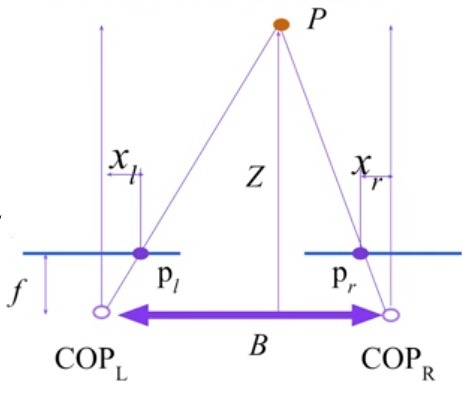
\includegraphics[scale=0.5]{Recursos/stereoGeometry.jpg}
        \caption{Representación del modelo de ejes alineados en el plano}
        \label{estereoSystemParallel}
     \end{subfigure}
     \hfill
     \begin{subfigure}[b]{0.4\textwidth}
         \centering
        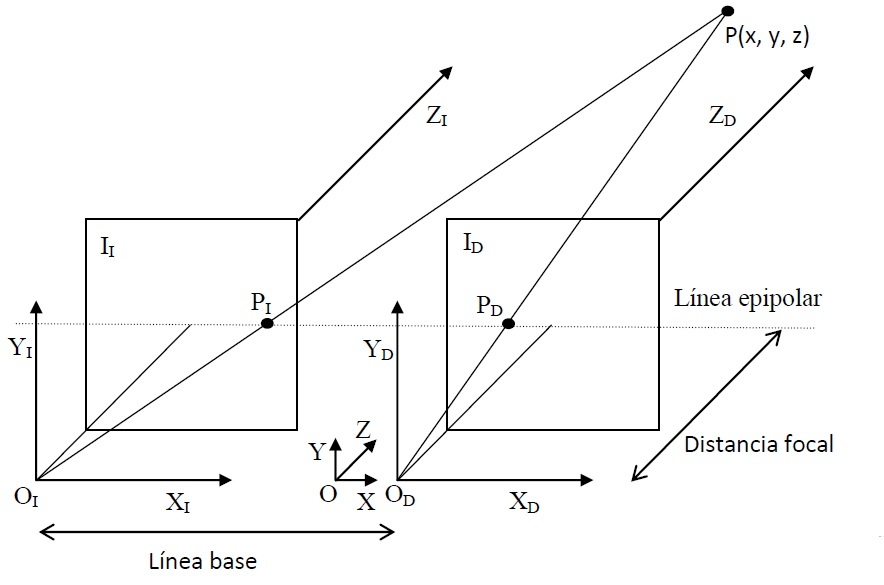
\includegraphics[scale=0.3]{Recursos/stereoGeometry3D.jpg}
        \caption{Representación del modelo de ejes alineados en el espacio}
        \label{estereoSystemParallel3D}
     \end{subfigure}
     \hfill
\caption{Modelo estéreo de ejes alineados}
\label{stereoMODEL}
\end{figure}
\section{Fundamentos del aprendizaje profundo o deep learning}
El aprendizaje profundo, es una rama del aprendizaje automático ó machine learning, que se caracteriza por poseer un conjunto de datos de entradas, ejemplos de una salida esperada por el sistema y una forma de medir cuando un algoritmo está realizando adecuadamente su trabajo, este último elemento es necesario, ya que permite determinar la distancia entre la salida actual del algoritmo y la salida esperada, la medición de la salida es usada como una señal de realimentación para así ajustar la forma en que el algoritmo funciona. A este ajuste se le conoce como ``aprendizaje''. Cabe destacar que cuando a un modelo de aprendizaje automático se le suministran las salidas esperadas pasa a ser parte de una sub-rama del aprendizaje profundo conocido como aprendizaje supervisado, pero no es una característica obligatoria del aprendizaje profundo suministrar la salida esperada, a esta otra sub-rama se le conoce como aprendizaje no supervisado.
\\
La idea base de este sub-campo del machine learning, nace del interés de replicar en sistemas computacionales el comportamiento de las neuronas presentes en los seres vivos, las cuales son responsables del aprendizaje y sus inicios datan de 1958 cuando Rosenblatt desarrollo el perceptron (Ver Figura \ref{perceptron}).
\begin{figure}[H]
    \centering
    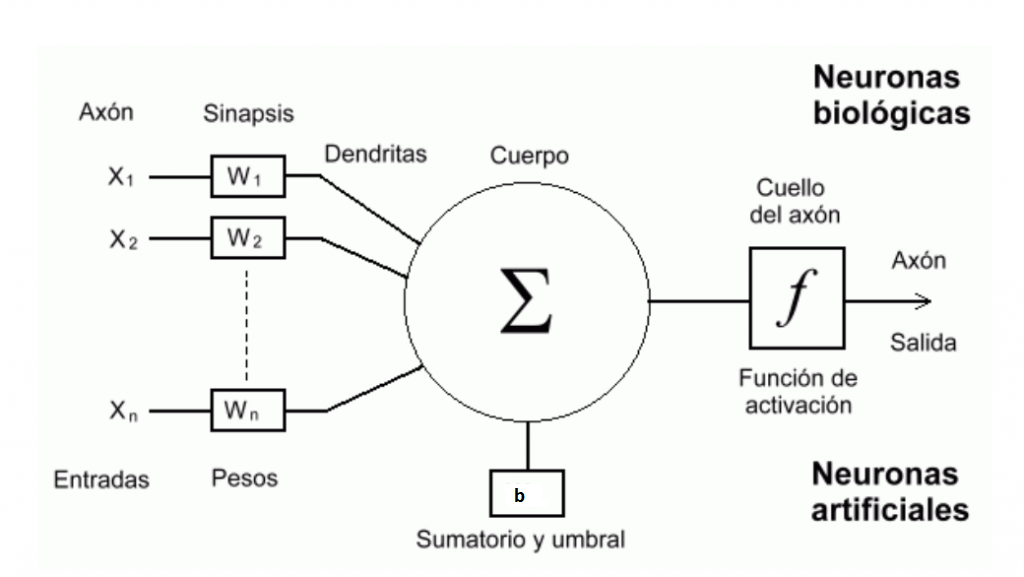
\includegraphics[scale=0.35]{Recursos/perceptron.png}
    \caption{Comparación de una neurona biológica con una neurona artificial}
    \label{perceptron}
\end{figure}
En comparación con otras técnicas de aprendizaje automático, que normalmente se basan en varias
etapas de preprocesamiento para extraer características en las que se pueden construir clasificadores, el enfoque de aprendizaje profundo
generalmente se entrena de un extremo a otro, yendo directamente desde píxeles sin procesar hasta los resultados finales deseados \cite{Szeliski2020}.
\subsection{Elementos de las redes neuronales}
\subsubsection{Pesos y capas}
Una red neuronal profunda extiende la idea del perceptron (Ver Figura \ref{perceptron}) que utiliza una única neurona, a un grafo compuesto por miles de neuronas interconectadas. En la Figura \ref{NeuralNetworkArq} cada circulo corresponde con una neurona cuya salida estará dada por la siguiente expresión:
\begin{equation}
    s_{i} = w_{i}^{T} x_{i} + b_{i} \label{ponderedSum}
\end{equation}
el resultado de las sumas ponderadas (ecuación \ref{ponderedSum}) de cada neurona pasa por una función de activación no linear que redistribuirá los valores en un rango acotado:
\begin{equation}
    y_{i} = h(s_{i})
\end{equation}
En la ecuación \ref{ponderedSum}, los valores de $x_{i}$ son las entradas de la i-esima neurona, $w_{i}$ y $b_{i}$ son parámetros que se van ajustando en el proceso de aprendizaje y corresponden con los pesos y el bias respectivamente. 
\begin{figure}[H]
    \centering
    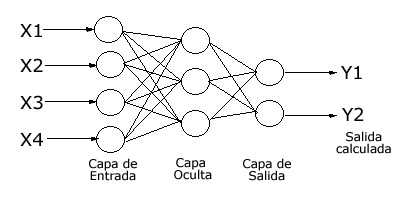
\includegraphics{Recursos/NeuralNetwork.jpg}
    \caption{Arquitectura de una red neuronal multicapas}
    \label{NeuralNetworkArq}
\end{figure}
A las capas de la Figura \ref{NeuralNetworkArq} se les conoce como ``fully conected'' (FC), debido a que todas las entradas de una capa están conectadas a todas sus salidas. Dado que las redes neuronales suelen estar organizadas en capas consecutivas, es posible agrupar cada neurona dentro de una capa en un vector, cuya combinación lineal se escribe como:
\begin{equation}
    s_{l} = w_{l}^{T} x_{l}
\end{equation}
donde $x_{l}$ son las entradas a la capa $l$, $W_{l}$ es una matriz de peso y $s_{l}$ es la suma ponderada, a la que se aplica una función de activación:
\begin{equation}
    x_{l+1} = y_{l} = h(s_{l})
\end{equation}
Una red que consiste únicamente en capas FC, se le conoce como perceptron multicapa. 
\subsubsection{Funciones de activación}
Las funciones de activación se usan para propagar la salida de los nodos de una capa hacia la siguiente capa. Además este tipo de funciones permiten incorporar al modelo no linealidades, que permitirán que este se ajuste a cualquier distribución de datos. Algunas de las funciones de activación más comunes son:
\begin{itemize}
    \item \textbf{función logística o sigmoidea:} Este tipo de funciones permiten mitigar el efecto de ``outliers'' (valores atípicos que son numéricamente distantes del resto de los datos) en el entrenamiento del modelo. La imagen de este tipo de funciones suele estar contenida en los intervalos [0, 1]. Por lo que valores muy extremos siempre estarán cerca de los límites del intervalo de esa imagen. Su ecuación está dada por:
    \begin{equation}
        h(x) = \frac{1}{1 + e^{-x}}
    \end{equation}
    \item \textbf{Tangente hiperbólica:} Es una función no lineal cuyo rango normalizado se encuentra entre [-1, 1] y su ventaja es que puede manejar más fácilmente los números negativos. Su ecuación está dada por:
    \begin{equation}
        h(x) = \frac{e^{x} - e^{-x}}{e^{x} + e^{-x}}
    \end{equation}
    \item \textbf{ReLu o rampa:} Es una de las funciones más utilizadas en redes convolucionales y en redes profundas debido a que con ella se logran mejores resultados que con la sigmoidea y la hiperbólica, ya que en el procesamiento de imágenes los valores negativos no son importantes y por lo tanto se establecen en 0. Pero los valores positivos después de la convolución deben pasar a la siguiente capa. En cambio si se emplean la hiperbólica o la sigmoidea, la información se pierde ya que ambas funciones modificarán las entradas a un rango muy cerrado. Su ecuación esta dada por:
    \begin{equation}
        h(x) = max(0,x)
    \end{equation}
\end{itemize}
\subsubsection{Funciones de error}
Como se ha podido observar el proceso de aprendizaje de una red neuronal es de carácter iterativo, ya que, lo que se busca es ajustar un modelo a un conjunto de datos. Las funciones de error permiten medir la distancia a la que se encuentra un modelo del objetivo, de esta forma es posible tomar medidas adecuadas en la siguiente iteración, para así reducir el error hasta alcanzar valores mínimos. Dependiendo de la tarea a realizar se utilizan diferentes funciones de error. 
\\
Por ejemplo, en el caso de redes que utilicen como datos de entrada mapas de profundidad (mapas de disparidad) ó imágenes sin ruido, se suele realizar una regresión matemática que ajuste al modelo, por lo que es común utilizar la norma L2 como función de error
\begin{equation}
    E(w) = \sum_{n} E_{n}(w) = - \sum_{n} ||y_{n} - t_{n}||^{2}
\end{equation}
donde $y_{n}$ es la salida de la red para la muestra n y $t_{n}$ es el valor objetivo. Sin embargo, si son pocos los ``outliers'' en los datos de entrenamiento, o si los errores graves no son tan dañinos como para merecer una penalización cuadrática, se pueden utilizar normas más robustas como la L1
\begin{equation}
    E(w) = \sum_{n} E_{n}(w) = - \sum_{n} ||y_{n} - t_{n}||
\end{equation}
Cabe resaltar que no son las únicas funciones de error utilizadas en el campo de visión estéreo, pues existen variaciones, como en el trabajo realizado por Sizhang Dai y Weibing Huang en marzo del 2020 \cite{dai2020atvsnet} donde usan el error absoluto medio.
\subsubsection{Técnicas para la optimización de la red}
Cuando se entrena una red se emplean diversas técnicas que mejoran los resultados de la misma, o permiten que las redes neuronales no sufran de ``overfitting'' (sobre ajuste) para así poder generalizar mejor. A continuación se detallaran algunas de las técnicas más empleadas así como lo es el ``dropout'' y la normalización del lote.
\begin{itemize}
    \item \textbf{Regularización:} es una técnica que surge cuando se optimizan los pesos dentro de una red neuronal, los pesos se vuelven más pequeños, a este fenómeno se le conoce como decaimiento de los pesos y es un problema debido a que al pasar por la función de activación un valor de suma ponderada muy cercano a 0, es mucho más difícil para el algoritmo del descenso al gradiente desplazar el valor de ese peso a su óptimo. En la práctica, valores muy pequeños se traducen a coeficientes con muchos decimales y esto es sinónimo de ``overfitting'', para solucionar esto se aplica regularización a la función de error, lo que penaliza en mayor medida a los pesos con largos coeficientes. A continuación se presentan las regularizaciones L1 y L2 respectivamente.
    \begin{align}
          E(w)_{L1} = - \sum_{n} ||y_{n} - t_{n}|| + \lambda \sum_{i} |w_{i}|\\
          E(w)_{L2} = - \sum_{n} ||y_{n} - t_{n}|| + \lambda \sum_{i} w_{i}^{2}\\
    \end{align}
    El valor de $\lambda$ corresponde con cuanto se quieren penalizar los coeficientes de los pesos $w_{i}$.
    \item \textbf{Dropout:} es una técnica aplicada a todas las neuronas de una capa, consiste en que a cada neurona de la capa en cuestión tendrá asociada una probabilidad de desactivación que puede estar entre 0 y 100\%, por lo que la red tendría un funcionamiento como el de la Figura \ref{dropout}.
    \begin{figure}[H]
        \centering
        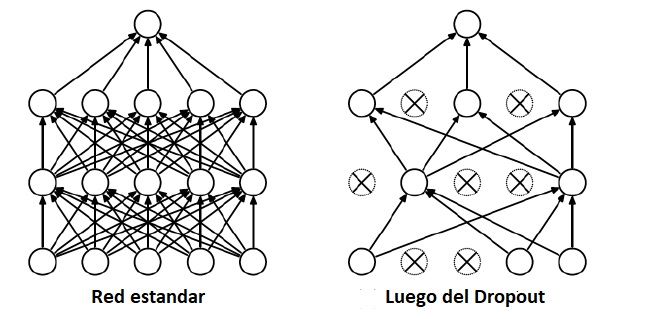
\includegraphics[scale=0.7]{Recursos/Dropout.jpg}
        \caption{Efecto del Dropout en el entrenamiento}
        \label{dropout}
    \end{figure}
    Colocar neuronas aleatoriamente a cero inyecta ruido en el proceso de formación y también evita que la red se especialice demasiado  sus neuronas a muestras o tareas particulares, de tal forma que se reduce el sobreajuste y mejorar la generalización.
    \item \textbf{Aumento del conjunto de datos:} Otra técnica poderosa para reducir el ajuste excesivo es agregar más muestras de entrenamiento perturbando las entradas y / o salidas de las muestras que ya han sido recolectadas. Esta técnica es eficaz en tareas de clasificación de imágenes, ya que es caro obtener ejemplos etiquetados, y también dado que las clases de imágenes no deben cambiar bajo pequeñas perturbaciones.
\end{itemize}
\subsubsection{Algoritmo de backpropagation}
Propuesto en 1986 por Rumelhart, Hinton y Williams, es el responsable de que una red neuronal sea capaz de auto ajustar sus parámetros para así aprender una representación interna de la información que estaba procesando. Para su ejecución se requiere de un algoritmo conocido como descenso al gradiente, el cual consiste en que en cada iteración del entrenamiento se evalúe el error del modelo y se calculen las derivadas parciales (gradientes) de dicho error, los gradientes indicaran la pendiente de la función hacia donde el error incrementa, por lo que para reducir el error en cada iteración, es necesario substraer el vector de gradientes al resultado final. 
\\
No obstante, debido a la estructura de una red neuronal, los valores de los parámetros en las capas posteriores dependen de las capas previas y a su vez de las conexiones entre neuronas, por lo que calcular el gradiente de forma directa no es una opción, la solución es utilizar el descenso del gradiente para optimizar la función de coste (función de error) empleando la técnica de backpropagation para calcular el vector de gradientes dentro de la complejidad de la arquitectura de la red. 
\\
El funcionamiento de este algoritmo parte de analizar desde el final de la red con la señal de error hacia las primeras capas, la razón del porqué se va desde la última capa hacia la primera capa, es que en una red neuronal el error de las capas anteriores depende directamente del error de las capas posteriores, teniendo en cuenta este hecho, es posible determinar cuál es el efecto de cada neurona en el resultado final mediante la retro propagación de errores, de este modo es posible computar cuanto hay que modificar cada parámetro en cada neurona. Además una vez aplicados los errores a las neuronas de la capa de turno se puede proceder a repetir el mismo proceso previo como si este fuera el error de la red; es decir, asumiendo que la capa de turno es la nueva última capa, así aplicar backpropagation es operar siempre de forma recursiva capa tras capa moviendo el error hacia atrás. Entonces al alcanzar la primera capa se habrá obtenido cuál es el error para cada neurona y para cada uno de sus parámetros, dichos errores son usados para calcular las derivadas parciales de cada parámetro de la red, conformado así el vector de gradientes al cual se le aplica el descenso al gradiente para lograr minimizar el error. 
\subsection{Redes neuronales convolucionales ó Convolutional Neural Networks (CNN)}
Es una arquitectura de red empleada en el procesamiento de imágenes, cuya principal ventaja respecto a las redes estudiadas previamente, es su eficiencia al momento del entrenamiento, ya que la cantidad de parámetros a ajustar se reduce considerablemente. A diferencia de una red de capas FC las capas de las redes CNN consisten en un conjunto de filtros que se van ajustando a medida que avanza el aprendizaje, cada filtro suele ser pequeño espacialmente (tanto en ancho como en alto) respecto a las dimensiones de la imagen de entrada, pero estos se extienden a través de todas las dimensiones del volumen de entrada, se le conoce como volumen de entrada debido a que una imagen con los 3 canales (RGB) corresponde con un tensor de dimensiones $WxHxD$ (ancho x alto x profundidad). Al introducir una imagen en la red se desliza (más precisamente, se realiza la convolución) cada filtro a través de todo el ancho y alto del volumen de entrada y se calculan los productos escalares entre las entradas del filtro y la entrada en cualquier posición.  A medida que se desliza el filtro sobre el ancho y el alto del volumen de entrada, se producirá un mapa de activación bidimensional o mapa de características, que da las respuestas de ese filtro en cada posición espacial (Ver Figura \ref{fowardPassCNN}).
\begin{figure}[H]
    \centering
    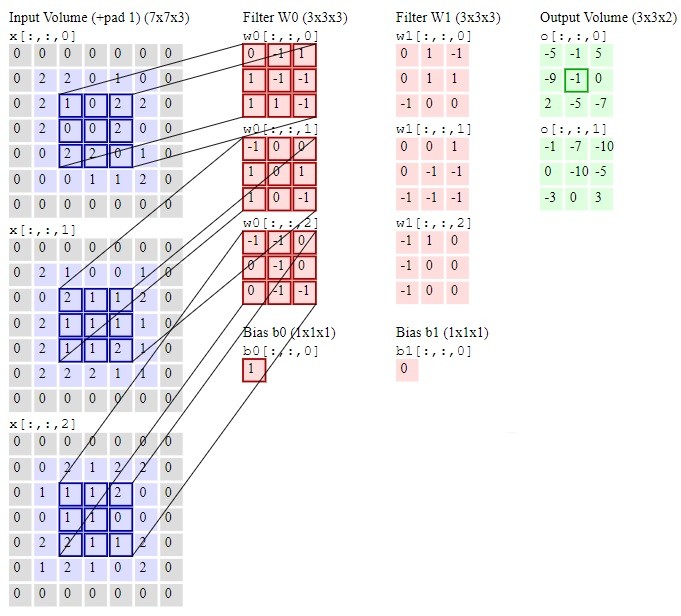
\includegraphics[scale=0.7]{Recursos/fowardPassCNN.jpg}
    \caption{Convolución entre el volumen de entrada de dimensiones 7x7x3 y dos filtros de dimensiones 3x3x3}
    \label{fowardPassCNN}
\end{figure}
De forma intuitiva, la red aprenderá filtros que se activan cuando ven algún tipo de característica visual, como un borde de alguna orientación o una mancha de algún color en la primera capa, o eventualmente patrones enteros en forma de panal o rueda en capas superiores de la red. De este modo se tendrá un conjunto completo de filtros en cada capa, en lugar de neuronas y cada uno de ellos producirá un mapa de activación bidimensional separado. Se Apilaran estos mapas de activación a lo largo de la dimensión de profundidad generando así el volumen de salida\cite{CS231n}.
\\ 
En las CNN se suelen emplear dos tipos de capas, aquellas donde se realiza la convolución, las cuales fueron descritas previamente y las capas de agrupación o ``polling layers'', estas son insertadas periódicamente entre capas de convolución con el fin de reducir progresivamente el tamaño espacial de la representación para así disminuir la cantidad de parámetros y cálculos en la red y, por lo tanto, controlar también el ``overfitting''. La capa de agrupación funciona de forma independiente en cada segmento de profundidad de la entrada y la redimensiona espacialmente, utilizando la operación MAX. La forma más común es una capa de agrupación con filtros de tamaño 2x2 aplicados con un paso de 2, por lo que con estos parámetros la operación MAX tomaría el valor máximo entre 4 números en una región de 2x2 (Ver Figura \ref{maxPooling}). De manera más general, la capa de agrupación:
\begin{itemize}
    \item Acepta un volumen de dimensiones $W_{1}xH_{1}xD_{1}$
    \item Requiere dos hiperparámetros:
    \begin{itemize}
        \item Su extensión espacial ``F''
        \item El paso o zancada ``S''
    \end{itemize}
    \item Produce un volumen $W_{2}xH_{2}xD_{2}$.
    \item Introduce cero parámetros, ya que calcula una función fija de la entrada
    \item Para las capas de agrupación, no es común rellenar la entrada con relleno (padding) de ceros, como en el caso de una capa de convolución.
\end{itemize}
\begin{figure}[H]
    \centering
    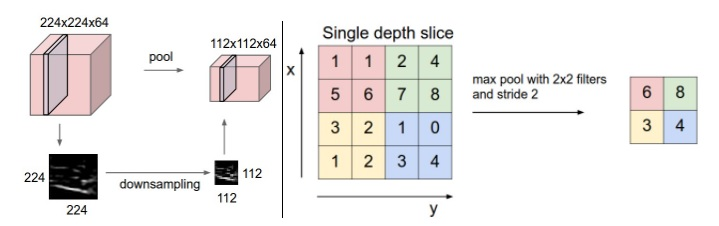
\includegraphics[scale=0.6]{Recursos/maxPolling.jpg}
    \caption{Capa de agrupación para un volumen de entrada de 224x224x64 con F = 2, P = 2 y un volumen de salida de 112x112x32}
    \label{maxPooling}
\end{figure}
\subsection{Hiperparámetros de las redes CNN}
Son las variables que rigen el proceso de entrenamiento en sí, es decir; son variables de configuración. En el caso de las capas de convolución se tienen:
\begin{enumerate}
    \item La profundidad del volumen de salida: corresponde a la cantidad de filtros a usar en cada capa y se identifica por $D_{n}$ donde $n$ es el número de la capa en cuestión. Sin embargo, también puede identificarse mediante $K$.
    \item El campo receptivo de la neurona: es equivalente al tamaño del filtro y se identifica mediante $F$.
    \item El paso o zancada: corresponde con la cantidad de píxeles por las que se desliza el filtro al momento de realizar la convolución, se identifica mediante la letra $S$. Por ejemplo cuando el paso es 1, los filtros se desplazan un píxel a la vez. En el caso de ser 2 los filtros saltan 2 píxeles a la vez a medida que se deslizan por el volumen de entrada, de esta forma se producirán volúmenes de salida más pequeños espacialmente.
    \item El relleno: hay casos donde será conveniente rellenar el volumen de entrada con ceros alrededor del borde, como es el caso de la Figura \ref{fowardPassCNN}. Por lo tanto el tamaño del relleno de ceros es un hiperparámetro que  permitirá controlar el tamaño espacial de los volúmenes de salida, aunque su aplicación más común es la de preservar exactamente el tamaño espacial del volumen de entrada para que el ancho de entrada y salida y la altura sean los mismos.
    \item Dilatación: este parámetro permite tener filtros que tengan espacios entre cada celda, por ejemplo; en el caso de una dimensión un filtro $w$ de tamaño 3 calcularía sobre la entrada $x$ lo siguiente: $w [0] * x [0] + w [1] * x [1] + w [2] * x [2]$. Este es en el caso de que no exista dilatación (dilatación = 0). Para la dilatación = 1, el filtro calcularía $w [0] * x [0] + w [1] * x [2] + w [2] * x [4]$; En otras palabras, hay una brecha de 1 entre las aplicaciones.  Esto puede ser muy útil en algunas configuraciones para usar junto con filtros de dilatación 0 porque le permite fusionar información espacial a través de las entradas de manera mucho más agresiva con menos capas.
\end{enumerate}
De acuerdo con los hiperparámetros, una capa convolucional se caracteriza por:
\begin{itemize}
    \item Acepta un volumen de dimensiones $W_{1}xH_{1}xD_{1}$.
    \item Requiere 4 hiperparámetros:
    \begin{itemize}
        \item El numero de filtros ``K''
        \item La extensión de los filtros ``F''
        \item El paso ``S''
        \item la cantidad de relleno ``P''.
    \end{itemize}
    \item Produce un volumen $W_{2}xH_{2}xD_{2}$ donde:
    \begin{itemize}
        \item $W_{2}$ $=$ $(W_{1} - F + 2P)/S+1$
        \item $H_{2}$ $=$ $(H_{1} - F + 2P)/S+1$
        \item $D_{2}$ $=$ $K$
    \end{itemize}
\end{itemize}
\section{Detección de objetos usando YOLO}
Entre las formas de reconocimiento existentes basadas en redes neuronales You Only Look Once (YOLO) es una arquitectura de red capaz de conseguir una velocidad de predicción de 45 cuadros por segundo en su forma base y 155 cuadros con fast YOLO. Por otro lado, una cámara de teléfono captura vídeos alrededor de 30 cuadros por segundo, mientras que las cámaras de alta velocidad alcanzan alrededor de 250 cuadros por segundo. La velocidad de detección en milisegundos de YOLO está entre 6 a 22 ms, a comparación con el cerebro humano que es capaz de detectar alrededor de 13 ms. A este tipo de arquitectura se le introducen imágenes y entrega como resultado bounding boxes o cuadros delimitadores que engloban al objeto en cuestión y la clase a la que pertenece dicho objeto.
\\
\\
YOLO utiliza un elemento llamado intersección sobre la unión (IoU) para poder evaluar el grado de solapamiento entre una predicción y el ground truth (salidas esperadas etiquetadas a mano por seres humanos), dicha métrica está dada por la siguiente expresión: 
\begin{equation}
    IoU = \frac{\text{Área de solapamiento}}{\text{Área de unión}} = \frac{\text{Área común entre bounding boxes}}{\text{Área total cubierta por los bounding boxes}}
\end{equation}
En la Figura \ref{IoU} se puede apreciar un ejemplo de una IoU cercana a 0.9, debido a que el grado de solapamiento es bastante alto, en caso de que los dos bounding boxes no se solapen el IoU sería de 0, de no ser así dicha métrica alcanza un valor de 1. Esta es la forma de evaluar que tan buena es una predicción.
\begin{figure}[H]
    \centering
    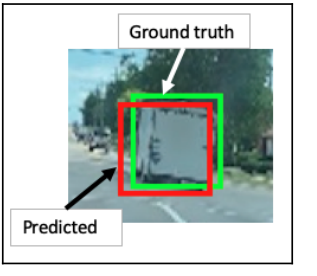
\includegraphics{Recursos/iou.png}
    \caption{IoU: Predicción vs. ground truth}
    \label{IoU}
\end{figure}
\subsection{Arquitectura de YOLOv3}
La versión número 3 de esta red tiene como base una CNN, que simultáneamente predice las coordenadas de múltiples bounding boxes y la probabilidad de detectar un objeto dado en cada bounding box.
\begin{figure}[H]
    \centering
    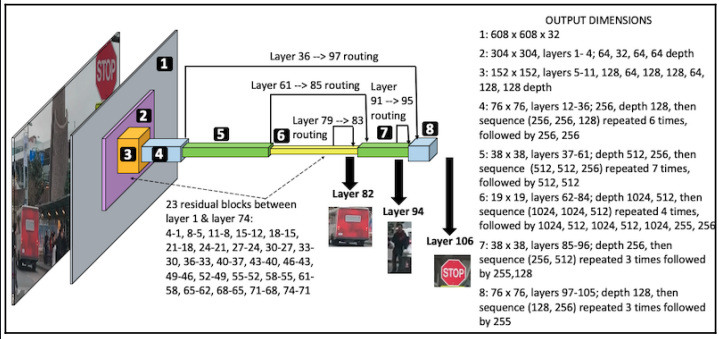
\includegraphics[scale=0.8]{Recursos/yolov3_architecture.png}
    \caption{Arquitectura de red YOLOv3. Imagen de \cite[p.~192]{Krishnendu}}
    \label{yolov3Architecture}
\end{figure}
 Esta versión del detector está compuesta por 24 capas convolucionales y dos FC (ver Figura \ref{yolov3Architecture}). Su mecanismo de detección es realizado a 3 diferentes escalas, específicamente en las capas 82, 94 y 106. La red utiliza 23 capas convolucionales y bloques residuales como los de la Figura \ref{tipos_de_bloques_residuales} entre las capas 1 y 74, donde el tamaño de la imagen de entrada cae de 608 a 19 píxeles y la profundidad aumenta de 3 a 1024 a través de los filtros alternos 3 x 3 y 1 x 1. El by-pass o salto de conexión característico de los bloques residuales ayuda a reducir el problema del desvanecimiento de los pesos al que se enfrentan las arquitecturas de redes profundas, lo que se traduce en que el algoritmo del descenso del gradiente pueda alcanzar su óptimo.
 \begin{figure}[H]
     \centering
     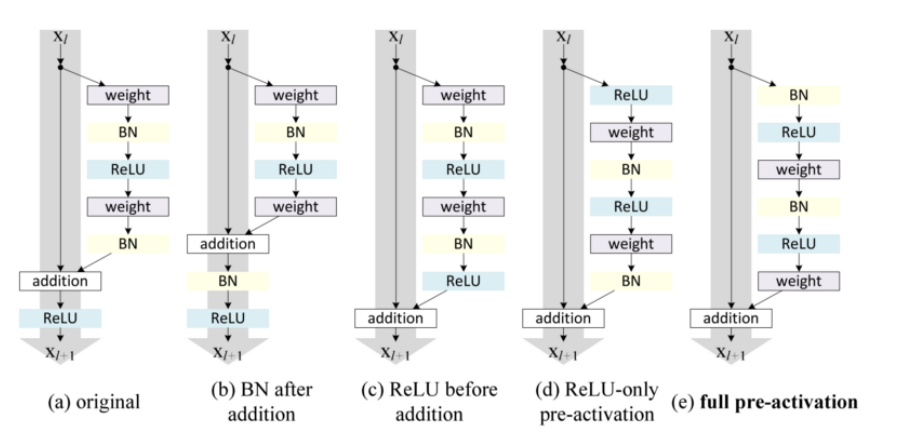
\includegraphics[scale=0.6]{Recursos/residual_block.png}
     \caption{Tipos de bloques residuales. Imagen de \cite{residualBlocksPaper}}
     \label{tipos_de_bloques_residuales}
 \end{figure}
Cada bloque residual empleado en esta arquitectura es sucedido por un bloque de pre-convolución de dimensiones 1 x 1 y filtros de dimensiones 3 x 3 hasta la primera detección en la capa 82. En la Figura \ref{yolov3Architecture} se observan dos saltos o by-passes, el primero entre las capas 61 a la 85 y el segundo entre la 36 a la 97. Así mismo, el paso o zancada se mantiene como 1 la mayor parte del tiempo, excepto en 5 casos, donde un valor de zancada de
2 se utiliza para la reducción de tamaño, junto con un filtro de 3 x 3.
\subsection{Funcionamiento}
A continuación se describirán de forma detallada los pasos que lleva a cabo esta arquitectura, para predecir los bounding boxes y la clase de uno o varios objetos en una imagen.
\begin{enumerate}
    \item La CNN en YOLO usa las características (features) de la imagen completa para predecir cada bounding box, por este motivo la predicción es global, en lugar de ser local.
    \item La imagen es dividida en celdas de una cuadrícula $S$ $x$ $S$, donde $S$ es una cantidad finita. Cada celda predice $B$ bounding boxes con una probabilidad ($P$). Entonces el número total de bounding boxes estará dado por $S$$x$$S$$x$$B$, con su correspondiente probabilidad para cada bounding box.
    \item Cada bounding box posee un vector de predicciones tal que, (x, y, w, h, c) el cual puede ser desglosado de la siguiente forma:
    \begin{itemize}
        \item (x, y): son las coordenadas del centro del bounding box, respecto a la coordenada de la celda ubicada en la cuadrícula.
        \item (w, h): son las dimensiones de ancho y alto respectivamente del bounding box en cuestión, respecto a las dimensiones de la imagen
        \item c: es el grado de confianza el cual representa el IoU entre la predicción y el ground truth.
    \end{itemize}
    \item La probabilidad de que una celda en la cuadrícula contenga un objeto, es definida por la probabilidad de que pertenezca a una clase dada multiplicada por el IoU, esto implica que si una celda contiene parcialmente a un objeto su probabilidad será baja y su valor de IoU se mantendrá bajo. Este hecho produce dos efectos en el bounding box de esa celda:
    \begin{itemize}
        \item La forma del bounding box será más pequeña que el tamaño del bounding box de la celda que incluye completamente el objeto porque la celda solo puede ver parte del objeto e infiere su forma a partir de ello. Además, si la celda contiene una parte muy pequeña del objeto no reconocerá el objeto del todo.
        \item El grado de confianza en la clase será pequeño debido a que el valor del IoU resultante de una imagen parcial no se ajustara con la predicción del ground truth.
    \end{itemize}
    \item En general, una celda puede contener solo una clase, pero usando el principio del ``anchor box'' múltiples clases pueden ser asignadas a una celda. Un anchor box como se puede ver en la Figura \ref{anchor_boxes} son regiones cuyas dimensiones son predefinidas por una expresión matemática o de acuerdo a la forma de la clase detectada. Por ejemplo: si se detectan tres clases como carro, motocicleta y humano, entonces es probable que utilizando dos anchor boxes, uno para humano y motocicleta y otro para el carro se logre la predicción deseada, esto se puede confirmar observando como en la Figura \ref{exampleYOLO} donde el objeto más a la izquierda corresponde con un carro. Para ajustar la forma de un anchor box sin emplear una ecuación matemática generadora se puede analizar la forma de cada clase en el conjunto de entrenamiento de la red usando algoritmos como "k-means clustering".
    \begin{figure}[H]
        \centering
        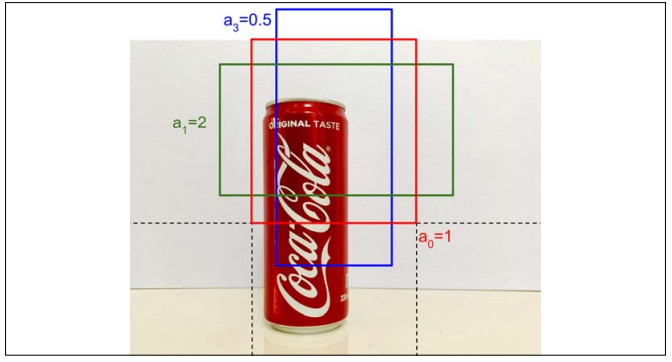
\includegraphics[scale=0.7]{Recursos/anchor_boxes.png}
        \caption{Anchor boxes para una región con relaciones de aspecto [1, 2, $\frac{1}{2}$]. Imagen de \cite[p.~376]{Atienza2018}}
        \label{anchor_boxes}
    \end{figure}
\end{enumerate}
En la Figura \ref{exampleYOLO} se tienen las tres clases ya mencionadas carro, motocicleta y humano asumiendo una cuadrícula de 5 x 5 con 2 anchor boxes y 8 dimensiones 5 para los parámetros del bounding box (x, y, w, h, c) y 3 para las clases (c1, c2, c3). Por lo tanto el vector de salida es 5 x 5 x 2 x 8.
\begin{figure}[H]
    \centering
    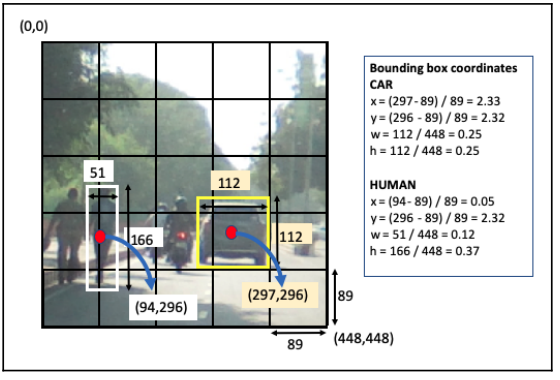
\includegraphics{Recursos/grid_example.png}
    \caption{Cálculo de las coordenadas de la predicción. Nota: el tamaño de la imagen es 448 x 448 (solo con propósitos de ilustración), se muestra el método de cómputo de las clases humano y carro y cada anchor box tiene un tamaño que puede ir desde 448/5 hasta 89 píxeles. Imagen de \cite[p.~191]{Krishnendu}}
    \label{exampleYOLO}
\end{figure}
\section{Segmentación}
Es un método de reconocimiento enfocado en clasificar cada píxel de una imagen de acuerdo a una clase correspondiente. Los algoritmos de segmentación fragmentan una imagen en conjuntos de píxeles o regiones con el propósito de tener un mejor entendimiento de lo que representa la imagen. De este modo el campo de la segmentación cambia dependiendo de la aplicación, los 3 casos más comunes son los siguientes:
\begin{itemize}
    \item \textbf{Segmentación de instancias:} se utiliza cuando el punto de interés son objetos contables dentro de una imagen, por lo tanto el resto de los objetos que no son de interés son clasificados como fondo o ``background'', tal es el caso de la Figura \ref{instance_segmentation}.
    \begin{figure}[H]
        \centering
        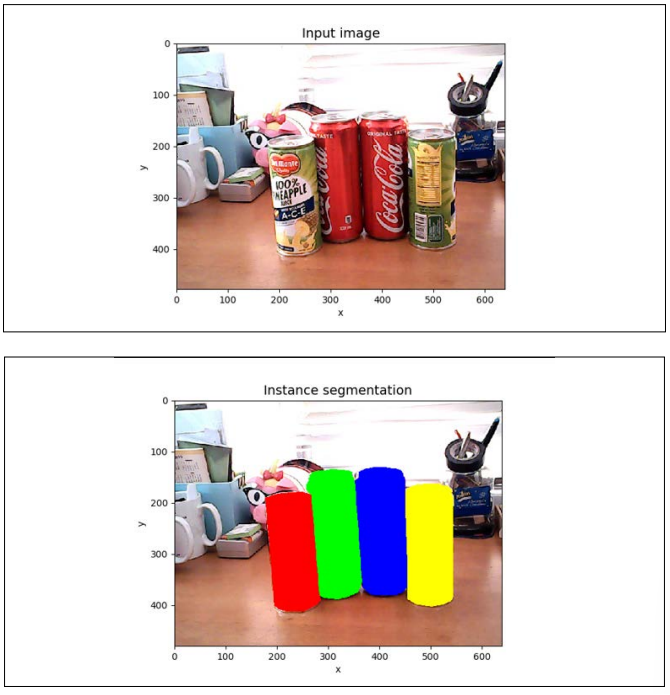
\includegraphics[scale=0.5]{Recursos/instance_segmentation.png}
        \caption{Ejemplo de segmentación de instancias. Imagen de \cite{Atienza2018}}
        \label{instance_segmentation}
    \end{figure}
    \item \textbf{Segmentación semántica:} cuando el centro de atención no son objetos contables, sino más bien regiones amorfas difíciles de contar como el cielo, bosques, vegetación, caminos, grama, edificios, etc.
    \item \textbf{Segmentación panóptica:} cuando se clasifican tanto los objetos contables como no contables es decir la imagen completa.
\end{itemize}
Como se pudo observar existen una gran variedad de técnicas cuando de segmentación se habla, aunque entre ellas la segmentación semántica se hizo bastante popular debido al modelo de código abierto desarrollado por Google ``DeepLab'' y su amplio campo de aplicación.
\subsection{Segmentación semántica con DeepLab}
En general posee una arquitectura basada en un encoder-decoder, mientras que el encoder toma la imagen de entrada (Ver Figura \ref{encoder_decoder}) para generar un vector de características, el decoder realiza el procedimiento inverso generando una imagen a partir de dicho vector. 
\begin{figure}[H]
    \centering
    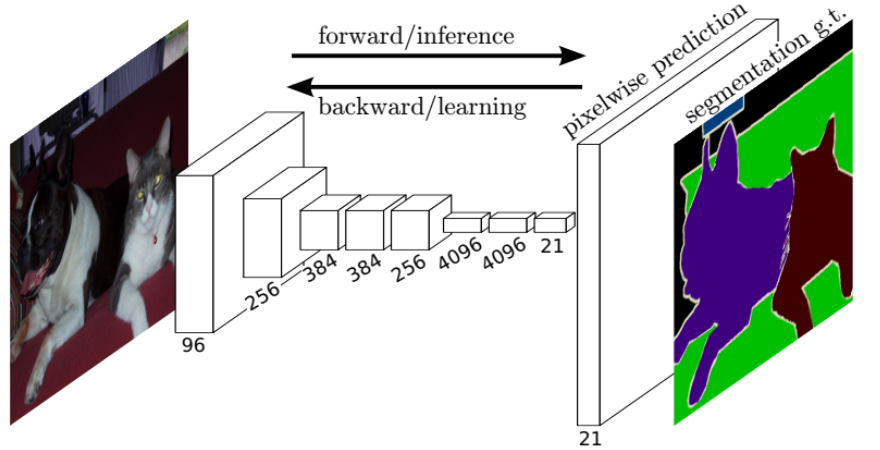
\includegraphics[scale=0.6]{Recursos/encoder_decoder.png}
    \caption{Arquitectura de DeepLab, Imagen de \cite{fullyConectedNet}}
    \label{encoder_decoder}
\end{figure}
Las características claves del encoder empleado son:
\begin{itemize}
    \item Emplea convoluciones dilatadas para extraer las características en las imágenes de entrada, estas como se puede ver en la Figura \ref{dilated_convolution} incrementan el campo de visión de la convolución. Mientras que una convolución normal emplea la zancada y capas de agrupación para reducir las dimensiones de salida de las capas, reduciendo la así la resolución de los mapas de características, lo cual es negativo para la segmentación, este método soluciona dicho problema. 
    \begin{figure}[H]
        \centering
        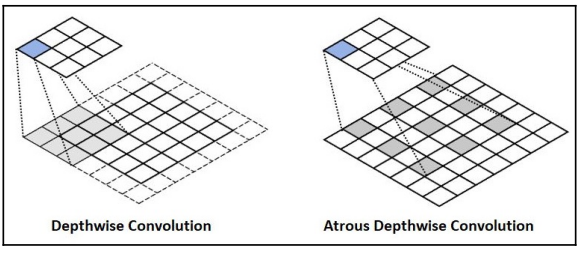
\includegraphics[scale=0.6]{Recursos/atrous_convolution.png}
        \caption{Comparación entre convolución común (izquierda) y convolución dilatada (derecha). Imagen de \cite{Krishnendu}}
        \label{dilated_convolution}
    \end{figure}
    \item El paso o zancada de salida esta dado por la relación entre la resolución de la imagen de entrada y la salida final. Un valor típico para esto es 16 u 8, lo que resulta en features más densas.
    \item Un modulo ASPP (atrous spatial pyramid polling) usado para realizar la convolución a diferentes escalas. Compuesto por convoluciones dilatadas apiladas en paralelo una detrás de otra para formar una spatial pyramid polling (SPP).  
\end{itemize}
Por otro lado el decoder posee las siguientes características:
\begin{itemize}
    \item Utiliza una convolución de dimensiones 1 x 1 para reducir los canales de los mapas de características de bajo nivel (producidos por el encoder).
    \item Emplea convoluciones de dimensiones 3 x 3 para obtener una segmentación más nítida.
    \item El factor de re-escalado es de 4, es decir; las dimensiones de ancho y alto de una capa a otra se cuadruplican hasta alcanzar las dimensiones originales.
\end{itemize}
Al implementar esta arquitectura es común que el encoder sea una red pre-entrenada de clasificación como lo son VGG o ResNet, utilizar redes pre-entrenadas para reentrenarlas con otros propósitos es llamado ``transferencia de aprendizaje''. Al aplicar la transferencia el decoder puede concentrarse en proyectar las features de menor resolución producidas por el encoder en un espacio de mayor resolución, para así obtener una clasificación densa de píxeles y a su vez reducir el tiempo de entrenamiento considerablemente.